The given system of inequalities can be written in matrix form as
\begin{align}
    \myvec{-5 & -4 \\ 1 & 0 \\ 0 & 1}\vec{x} \succeq \myvec{-20\\1\\2}
\end{align}
Let the surplus vector be
\begin{align}
    \vec{u} &= \myvec{u_1\\u_2} \succeq 0
\end{align}
\begin{enumerate}
    \item 
    \begin{align}
        \myvec{-5 & -4 \\ 1 & 0}\vec{x} &\succeq \myvec{-20 \\ 1}
        \\
        \implies  \myvec{-5 & -4 \\ 1 & 0}\vec{x} &= \myvec{-20 \\ 1} + \vec{u}
    \end{align}
    resulting in 
    \begin{align}
        \vec{x} &= \myvec{-5 & -4 \\1 & 0}^{-1}\myvec{-20 \\ 1} + \myvec{-5 & -4 \\1 & 0}^{-1}\vec{u}
        \\
        \implies \vec{x} &= \myvec{1 \\\frac{15}{4}} + \myvec{0 & 1\\ \frac{-1}{4} & \frac{-5}{4}}\vec{u}   \label{/2/47eq1}
    \end{align}
    \item 
    \begin{align}
        \myvec{-3 & -2 \\ 0 & 1}\vec{x} &\succeq \myvec{-12 \\ 2}
        \\
        \implies  \myvec{-3 & -2 \\ 0 & 1}\vec{x} &= \myvec{-12 \\ 2} + \vec{u}
    \end{align}
    resulting in 
    \begin{align}
        \vec{x} &= \myvec{-5 & -4 \\0 & 1}^{-1}\myvec{-20 \\ 2} + \myvec{-5 & -4 \\0 & 1}^{-1}\vec{u}
        \\
        \implies \vec{x} &= \myvec{\frac{12}{5} \\2} + \myvec{\frac{-1}{5} & \frac{-4}{5}\\ 0 & 1}\vec{u} \label{/2/47eq2}
    \end{align}
\end{enumerate}
Now,solution region which is common to regions of eq. \eqref{/2/47eq1} and eq. \eqref{/2/47eq2},is given by
\begin{align}
    \boxed{\vec{x} = \myvec{1 \\ 2}+\myvec{0 & 1\\ \frac{1}{20} & \frac{-21}{20}}\vec{u}}
\end{align}
and plotted in Fig. \ref{/2/47fig:fig1}	
\begin{figure}[!ht]
\centering
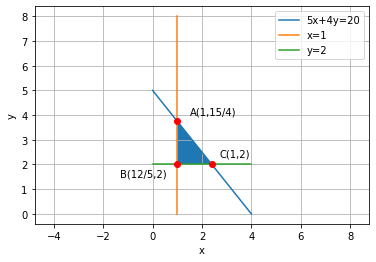
\includegraphics[width=\columnwidth]{solutions/su2021/2/47/ASSIGNMENT 11/SOLUTION.png}
\caption{Solution Region}
\label{/2/47fig:fig1}	
\end{figure}

